\section{Photonic Crystals}
A material with a periodically varying index of refraction with a period on the order of the wavelength of visible light is called a photonic crystal.
The first proposals for designing three-dimensional materials with such a property were published in 1987 by Yablonovitch \cite{Yablonovitch:1987p1809} and John \cite{John:1987}, but the study of naturally-occurring lower dimensional periodic structures can be traced to an 1885 publication by G. G. Stokes \cite{Stokes:1885}.
The theory of photonic crystals is often explained by analogy to electric semiconductors.
In a semiconductor, one solves the Schr\"{o}dinger equation for electrons in the material and finds that there is a range of energies that cannot propagate.
Similarly, in a photonic crystal, one solves Maxwell's equations given the spatial variations of index of refraction in the material and finds a range of frequencies that cannot propagate.
If there is a frequency range that cannot propagate in any direction the material is said to have a full photonic band gap.
If there is a frequency range that can propagate in some directions but not others the material has a partial photonic band gap \cite{Joannopoulos:2008p11516}.

If light of a frequency that is not allowed in a photonic crystal is incident upon the crystal in the appropriate orientation, conservation of energy requires that it be reflected.
When this frequency is in the visible, the crystal can appear brilliantly colored.
A naturally occurring example of this is found in opal gemstones.
Opals are composed of a crystalline packing of monodisperse silica spheres which have a size and index of refraction that is amenable to scattering visible light \cite{Sanders1968}.
While solving Maxwell's equations is the most fundamental method for determining which frequencies are not allowed, applying the conditions for Bragg diffraction is a simpler method that is effective for analyzing crystalline structures with easily identifiable lattice planes.
Bragg diffraction has been used to characterize atomic-scale crystal lattices by analyzing the constructive interference patterns of scattered X-rays which have wavelengths on the order of angstroms.
Constructive interference of visible light takes place when the material has lattice spacings on the order of hundreds of nanometers.
For a crystalline material with effective index of refraction, $n_e$, and a lattice spacing, $d$, the Bragg condition for constructive interference is 

\begin{equation}\label{eqn:Bragg} 
\lambda = 2n_edcos\theta, 
\end{equation}
where $\theta$ is the angle of incidence relative to the normal of the lattice plane and $\lambda$ is the wavelength of light in free space.
An illustration of the first few layers of a crystal of spheres and the relevant parameters for Bragg scattering is shown in Figure~\ref{fig:Bragg}a.
Figure~\ref{fig:Bragg}b shows an SEM image of a photonic crystal composed of 286 nm diameter polystyrene spheres embedded in silica.
The change in reflected color with angle of this sample is clearly seen in the photographs in Figure~\ref{fig:Bragg}c and d.

\begin{figure*}[htbp]
\centering
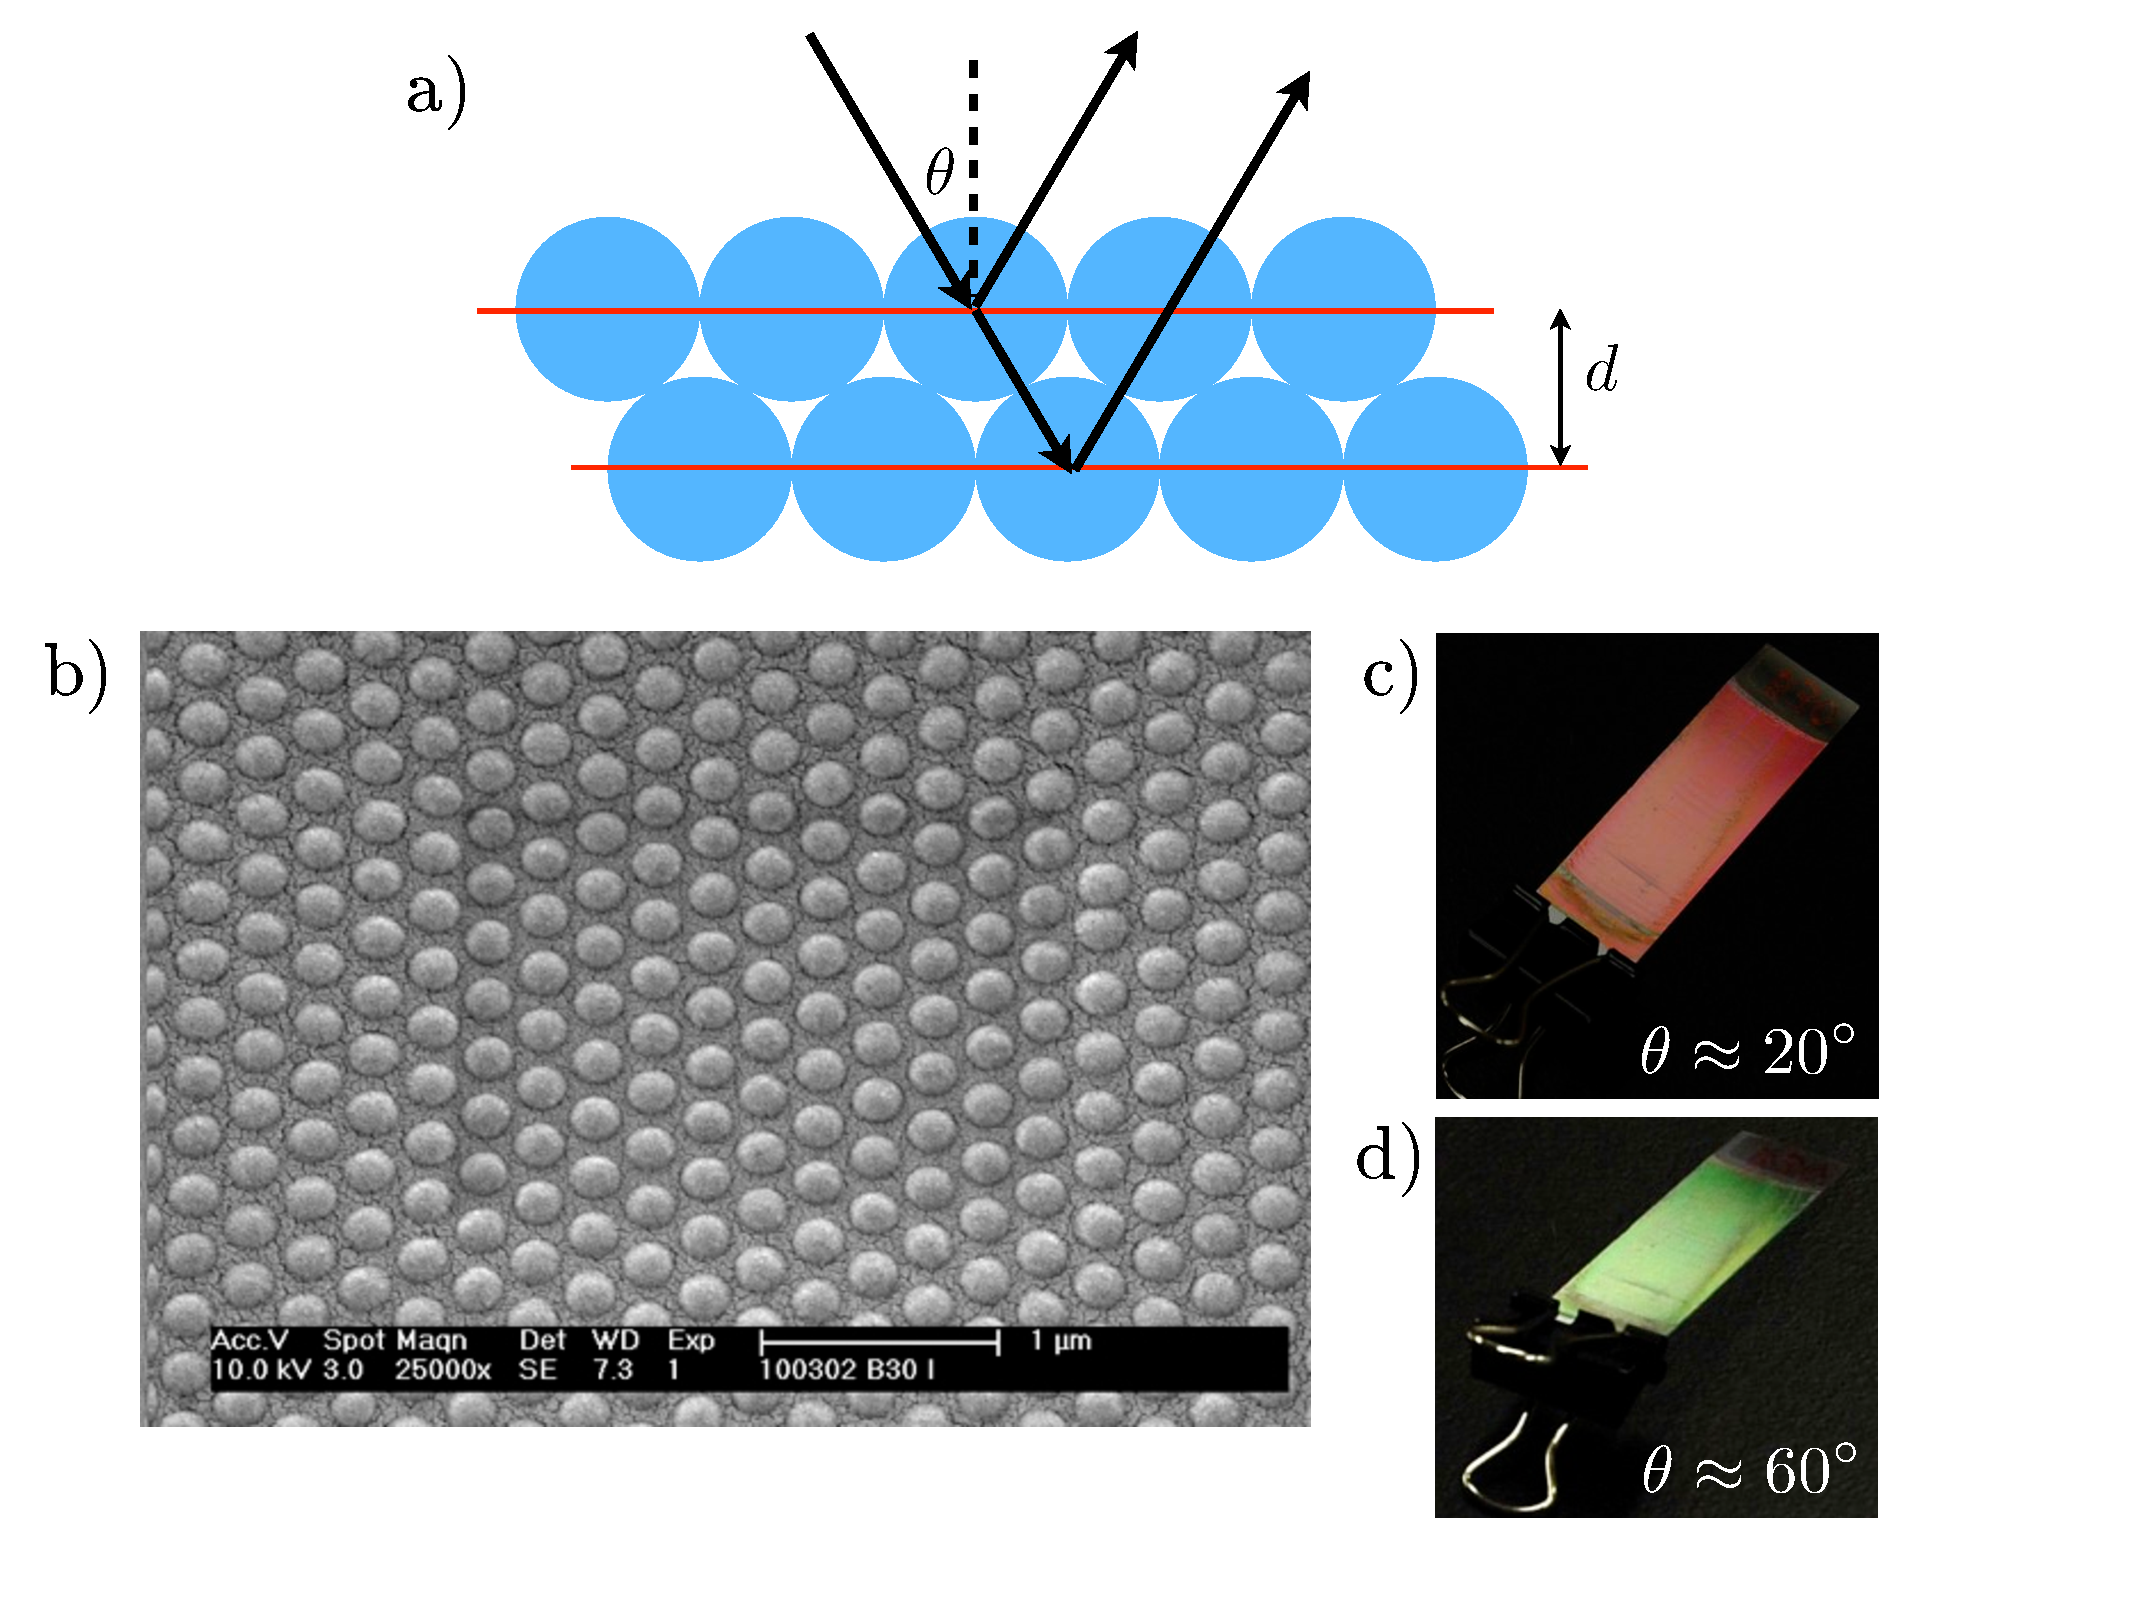
\includegraphics[width=0.9\textwidth]{figures/BraggWithRealCrystal.pdf}
\caption{\label{fig:Bragg} \emph{Photonic crystal and Bragg scattering.}
\emph{a)} Schematic for Bragg scattering.
\emph{b)} SEM image of the top layer of a polystyrene-in-silica photonic crystal. This sample was produced following the procedure described in Ref.~\cite{Hatton:2010}.
\emph{c)} Color photograph of a specular reflection from the sample in (b) inclined approximately 20$^{\circ}$ relative to a white light source.
\emph{d)} Color photograph of a specular reflection from the sample in (b) inclined approximately 60$^{\circ}$ relative to a white light source.
}
\end{figure*} 


In addition to the mineral example of opals there is a wide variety of photonic crystals found in the animal kingdom.
The colors of many butterfly and beetle scales and bird feathers are the result of scattering from crystalline structures produced by the organisms \cite{Vukusic:2003p1380, Welch:2007p1313,Srinivasarao:1999p9327}.
One striking feature of these kinds of structures is their iridescence --- their color changes as they are observed from different directions or in different lighting conditions.
The cause of this is readily apparent from Equation~\ref{eqn:Bragg}.
For a given lattice spacing, the wavelength of light that constructively interferes is a function of $\theta$ and when illuminated by white light, the apparent color of the feather or scale changes as its orientation changes.
Typically, the term \emph{photonic crystal} is used to describe man-made materials, while \emph{structural color} is used to describe biological examples because it emphasizes the fact that the color is the result of scattering, as opposed to absorption from a dye molecule.
Examining the structures responsible for these iridescent colors reveals a variety of exotic structures that are frequently more complicated than the packings of spheres that make up an opal \cite{Vukusic:2003p1380, Welch:2007p1313,Srinivasarao:1999p9327}.
All of them, however, are clearly periodic and applying the concept of Bragg scattering allows one to accurately predict the resulting color from knowledge of the physical structure.
Interestingly, there exist many examples of structural colors in bird feathers that are not iridescent \cite{Prum:1998p1228, Saranathan:2011}.
The microscopic structures in these feathers appear disordered and yet this structure is responsible for the color of the feathers.
Without clearly identifiable lattice planes we cannot use Bragg scattering to explain this structural color phenomenon.


\section{Avian Inspiration}

\begin{figure*}[htbp]
\centering
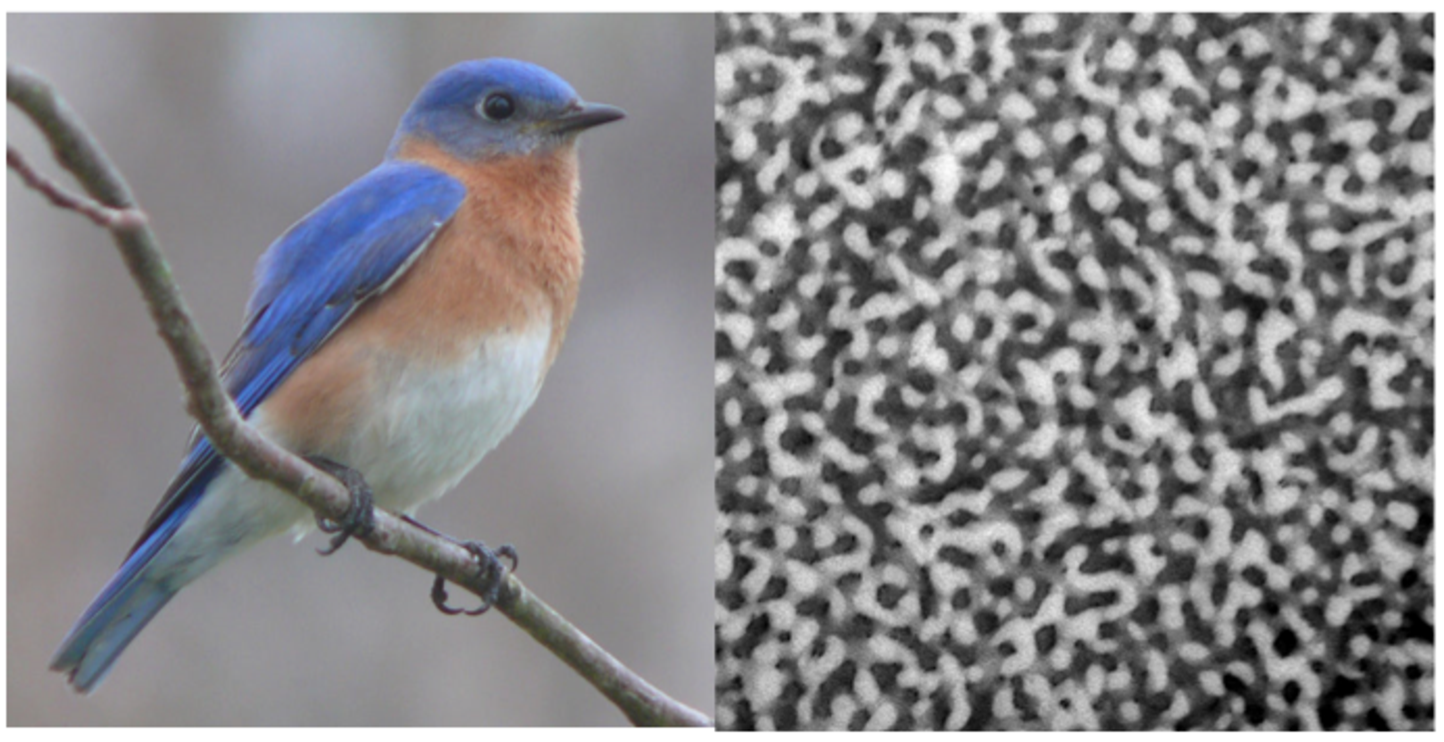
\includegraphics[width=0.9\textwidth]{figures/SialiaPic.pdf}
\caption{\label{fig:sialia} \emph{The eastern blue bird displays isotropic structural color.}
	\emph{Left panel:} Photograph of \emph{Sialia sialis}.
	\emph{Right panel:} TEM image of the channel-type structure responsible for the blue color of \emph{S. sialis}.
	The light regions correspond to air channels and the dark regions correspond to $\beta$-keratin.
	The field of view is 4.5 $\mu$m across.
	\emph{Note:} The reddish color of the chest feathers is not a structural color, it is the result of an absorbing dye.
	From Ref.~\cite{Dufresne:2009p6342}.}
\end{figure*}

\begin{figure*}[htbp]
\centering
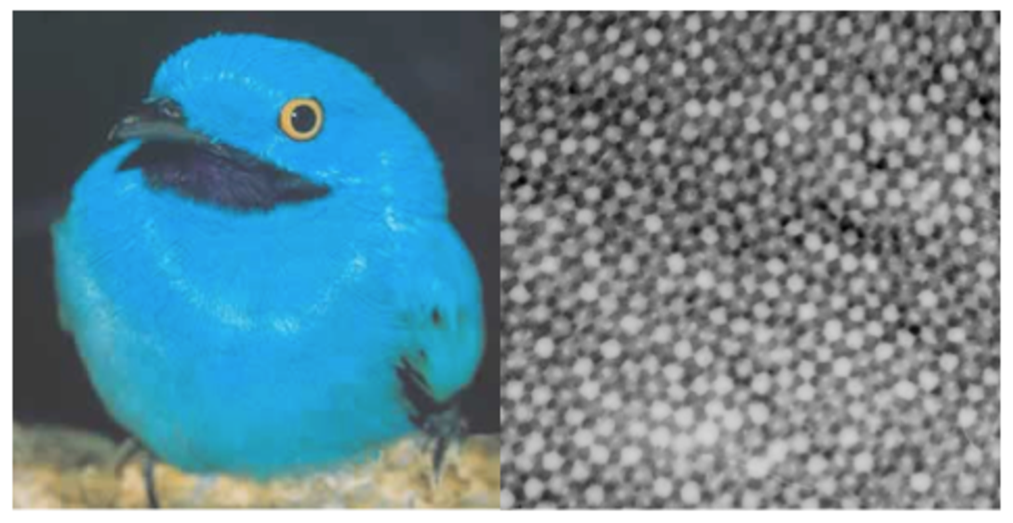
\includegraphics[width=0.9\textwidth]{figures/CotingaPic.pdf}
\caption{\label{fig:cotinga} \emph{The plum-throated cotinga displays isotropic structural color.}
	\emph{Left panel:} Photograph of \emph{Cotinga maynana}.
	\emph{Right panel:} TEM image of the sphere-type structure responsible for the blue color of \emph{C. maynana}.
	The light regions correspond to air pockets and the dark regions correspond to $\beta$-keratin.
	The field of view is 4.5 $\mu$m across.
	From Ref.~\cite{Dufresne:2009p6342}.}
\end{figure*}

\begin{figure*}[htbp]
\centering
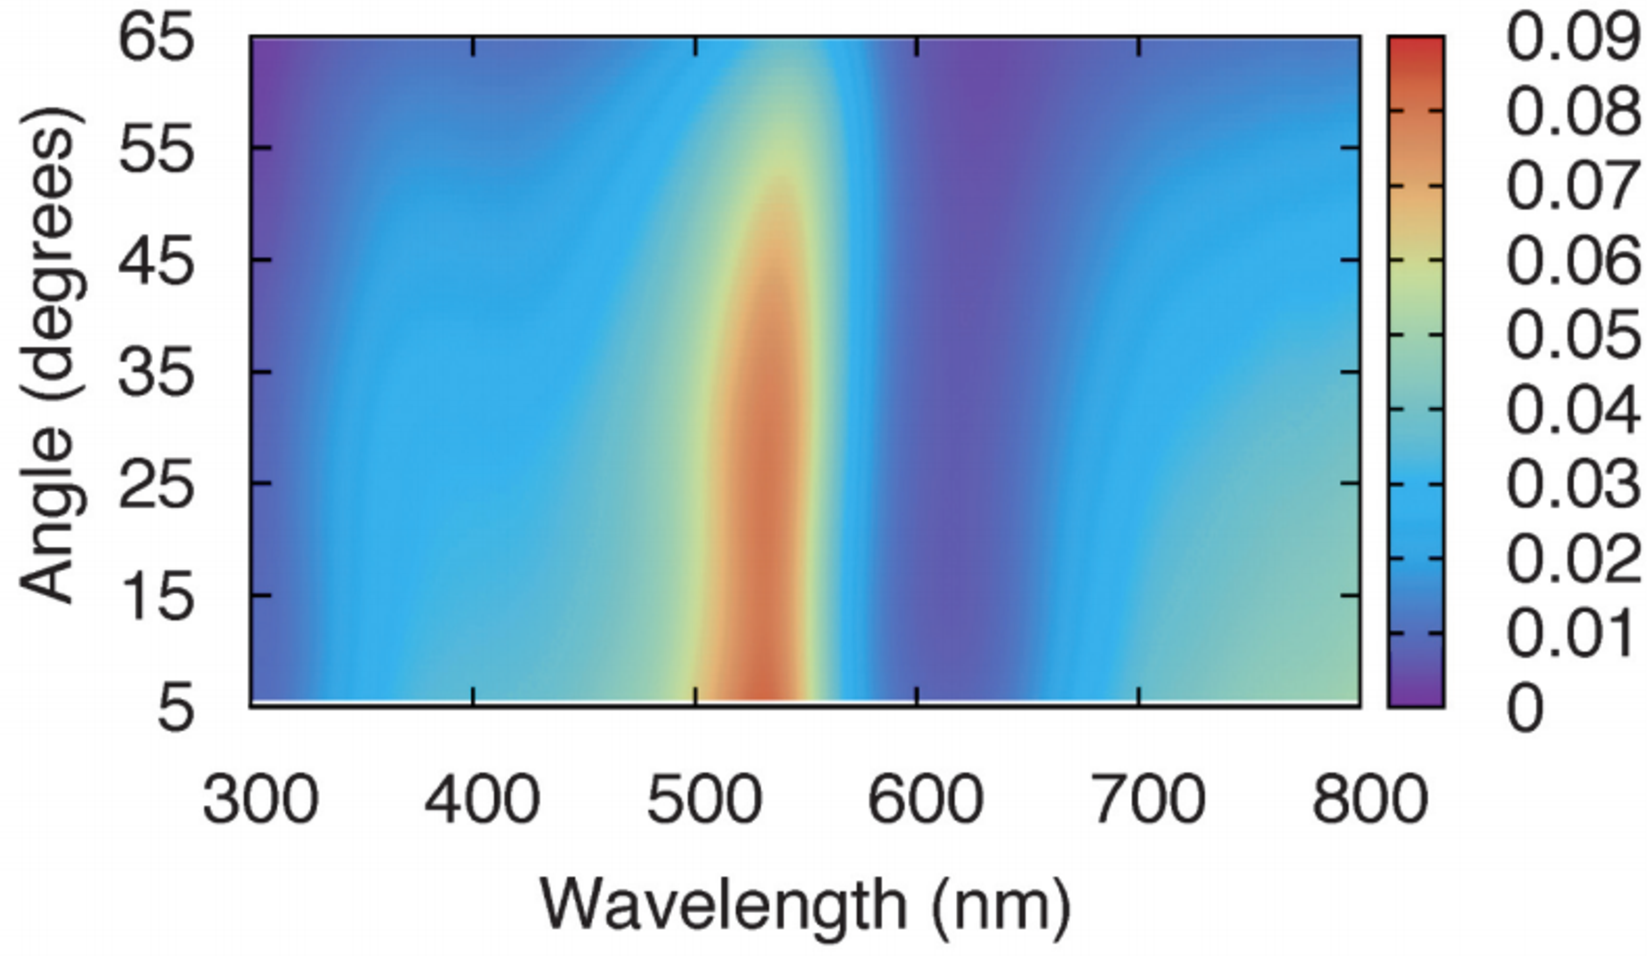
\includegraphics[width=5.0in]{figures/cmaynanaOpticalSpectra.pdf}
\caption{\label{fig:cotingaoptical} \emph{Angle-resolved optical reflection spectra from C. maynana}.
	From Ref.~\cite{Dufresne:2009p6342}.}
\end{figure*}

Many species of birds have feathers that are brilliantly-colored without the use of pigments.
Perhaps the most striking examples of structural color in nature are the iridescent colors created by scattering from periodic structures. 
Nature, however, also produces structural colors that have very little angle dependence.
These colors are the result of scattering from isotropic structures \cite{Dufresne:2009p6342, Prum:2009p3119, Prum:1998p1228}. 
Isotropic structural colors of bird feathers are produced by one of two classes of structures.
One class is a bi-continuous network of air and $\beta$-keratin, which is called channel-type. 
An example of the channel-type structure is found in the eastern blue bird (\emph{Sialia sialis}) and is shown in Figure~\ref{fig:sialia}.
The other class is an array of spherical air pockets in a background of $\beta$-keratin, which we call sphere-type.
The plum-throated cotinga (\emph{Cotinga maynana}) has feathers with the sphere-type structure and is shown in Figure~\ref{fig:cotinga}.
Neither the channel- nor sphere-type structure has obvious lattice planes that we could use to predict their colors via Bragg scattering.
Yet, as we can see in the reflection spectra recorded from \emph{C. maynana} in Figure~\ref{fig:cotingaoptical}, the peak wavelength is not sensitive to the angle of observation.
The question is then, how can these structures be responsible for scattering a narrow range of wavelengths?
To answer this question, we need a method to quantify the 3D architecture of these structures.

\begin{figure*}[htbp]
\centering
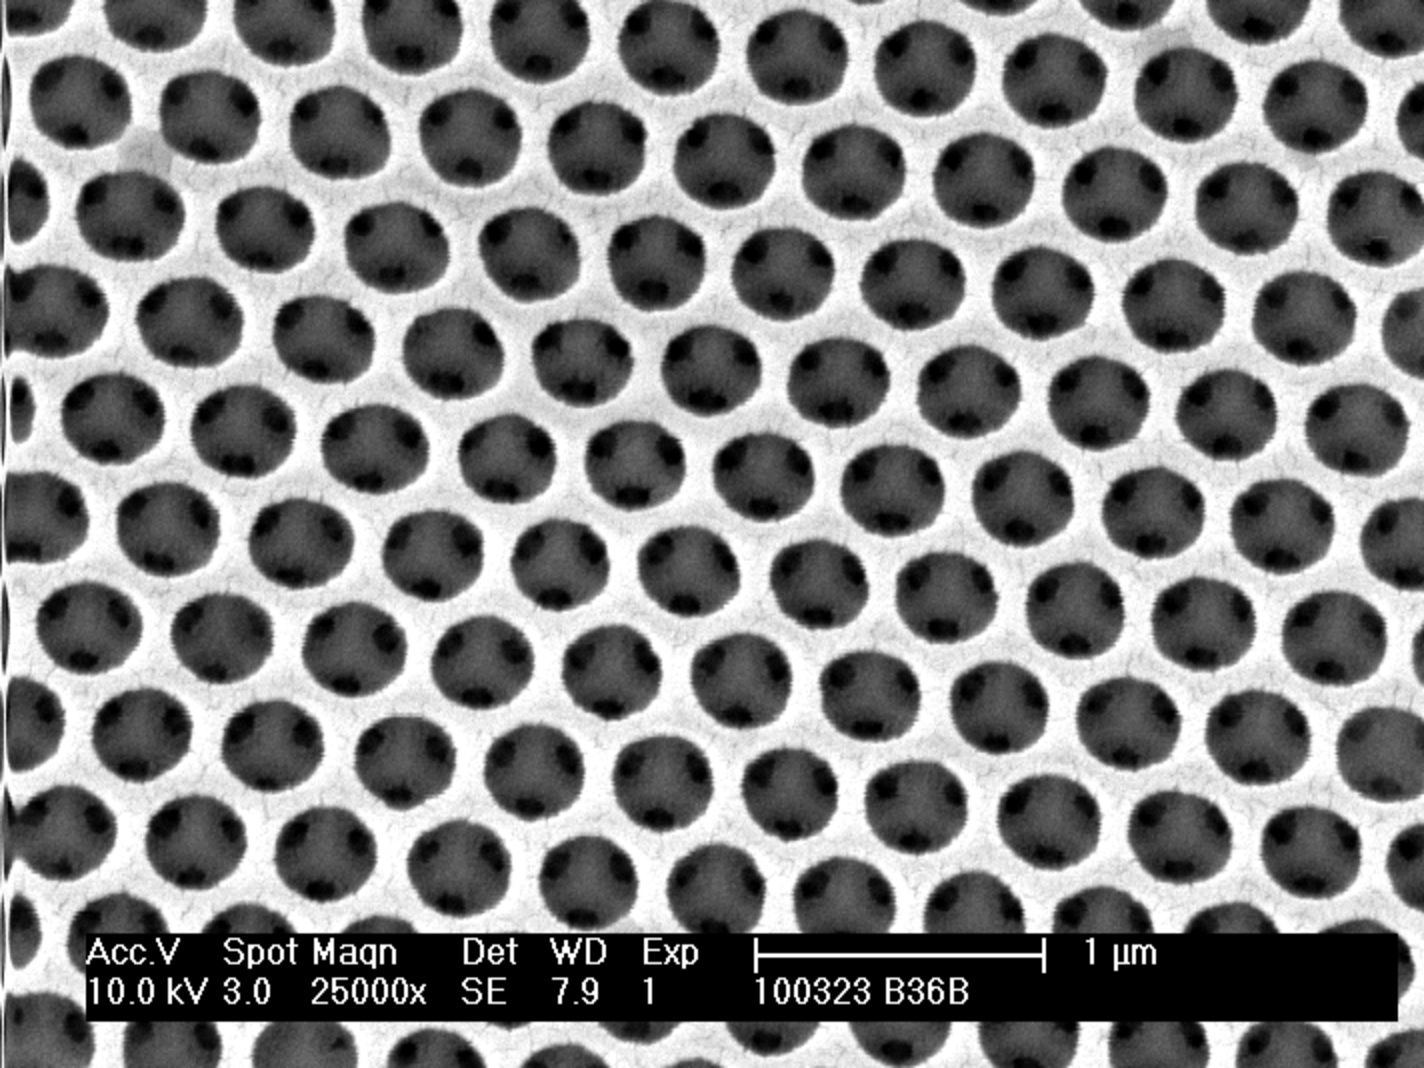
\includegraphics[width=3in]{figures/B36TEOSBurnedOut.pdf}
\hspace{0.5in}
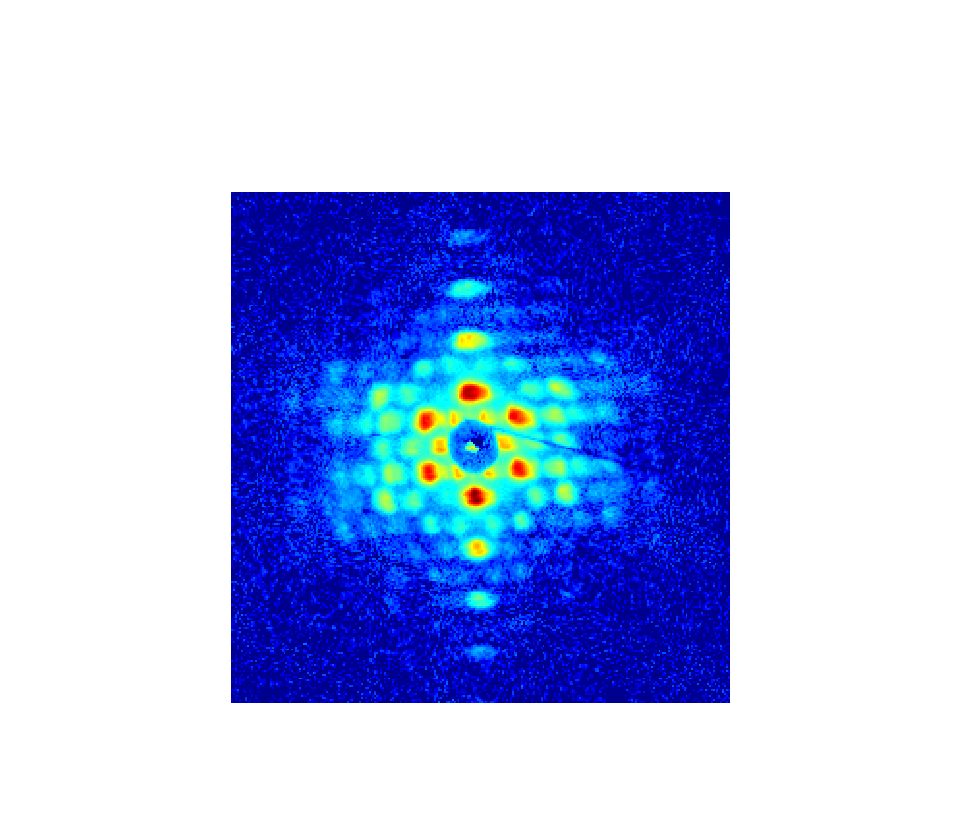
\includegraphics[width=2.25in]{figures/B36InvertedSAXS.pdf}
\caption{\label{fig:crystalSAXS} \emph{SAXS pattern from a hexagonal crystal has hexagonal symmetry.}
	\emph{Left panel:} SEM image of an air-in-silica crystalline structure produced via a colloidal template following the procedure described in Ref.~\cite{Hatton:2010}.
	\emph{Right panel:} SAXS pattern from the structure in the left panel. The hexagonal symmetry of the spots is a result of the hexagonal symmetry of the structure. The radial positions of the spots correspond to the lattice spacings in the structure. The log of intensity is plotted to improve contrast. The entire width of the image represents 0.43 nm$^{-1}$.}
\end{figure*}

\begin{figure*}[htbp]
\centering
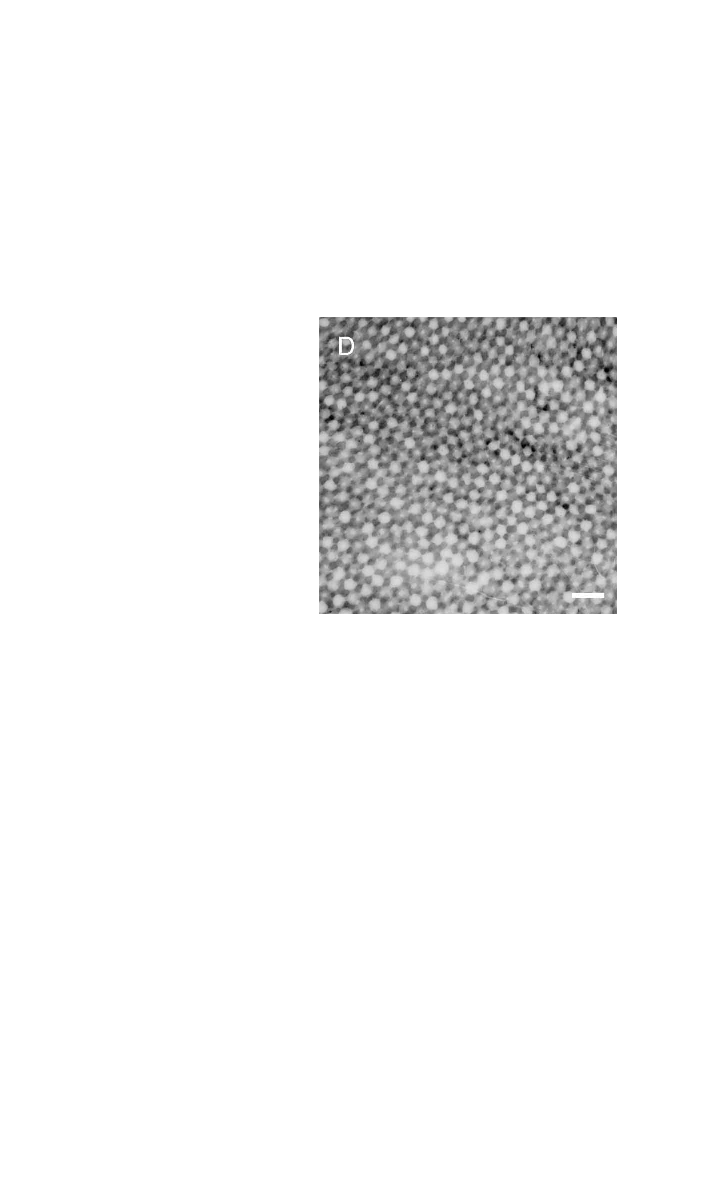
\includegraphics[width=2.5in]{figures/cmaynanaTEM.pdf}
\hspace{0.5in}
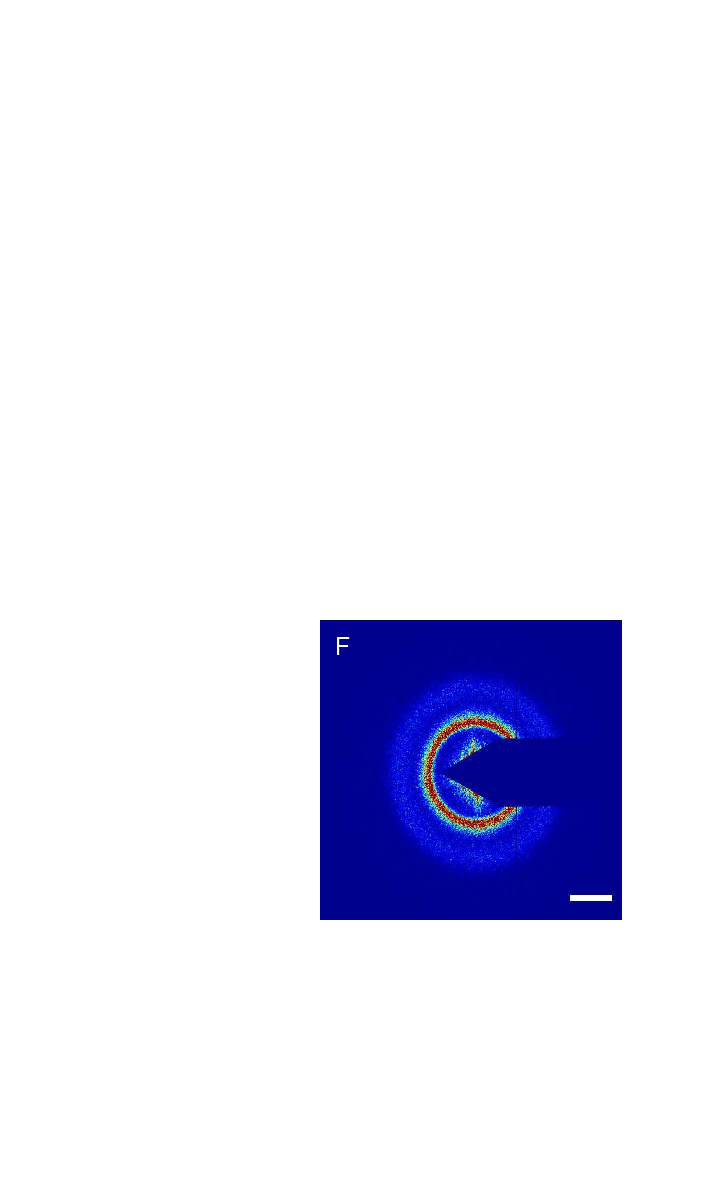
\includegraphics[width=2.5in]{figures/cmaynanaSAXS.pdf}
\caption{\label{fig:cotingaSAXS} \emph{SAXS pattern from an isotropic structure is a ring of uniform intensity.}
	\emph{Left panel:} TEM image of the color-producing structure in the feathers of \emph{C. maynana}.
	The scale bar represents 500 nm.
	\emph{Right panel:} SAXS pattern from the structure on the left.
	The scale bar represents 0.025 nm$^{-1}$.
	From Ref.~\cite{Dufresne:2009p6342}.}
\end{figure*}

The most fruitful technique we have employed in the characterization of these structures is small angle X-ray scattering (SAXS).
SAXS involves imaging the scattering pattern produced as a collimated beam of X-rays is passed through the structure of interest.
The scattering pattern contains a wealth of structural information: the radial position of a region of high intensity corresponds to a characteristic length scale in the scattering structure while the azimuthal distribution of intensity corresponds to symmetries in the structure.
The scattering pattern produced by a crystalline material with grain sizes that are comparable to or larger than the spot size of the X-ray beam will consist of a set of bright spots, the radial positions of which correspond to the lattice spacing in the crystal and the symmetry of which correspond to the symmetry of the crystal structure.
An example SAXS pattern from a photonic crystal is shown in Figure~\ref{fig:crystalSAXS}.
In this case, a hexagonal crystal of air spheres in a silica background produces a scattering pattern with hexagonal symmetry.
In contrast, materials that have a characteristic length scale but no long-range translational order will produce a scattering pattern in the form of a ring with uniform azimuthal intensity.
The isotropic structure from \emph{C. maynana} and the corresponding SAXS pattern are shown in Figure~\ref{fig:cotingaSAXS}.
The radius of the ring corresponds to the size of a dominant spatial correlation in the material and the absence of discrete points indicates a lack of long-range translational order.
A crystalline material may produce a ring-like SAXS pattern if the grains are small compared to the beam size, but there are typically multiple well-defined rings, each corresponding to one of the various lattice spacings characteristic of the crystal structure.
X-ray powder diffraction is a technique that takes advantage of this fact to identify the crystal structure of a material with small crystal grains \cite{Pecharsky:2003}.
The pattern in Figure~\ref{fig:cotingaSAXS}, however, shows only two peaks and does not indicate the presence of any local crystalline order.

\begin{figure*}[htbp]
\centering
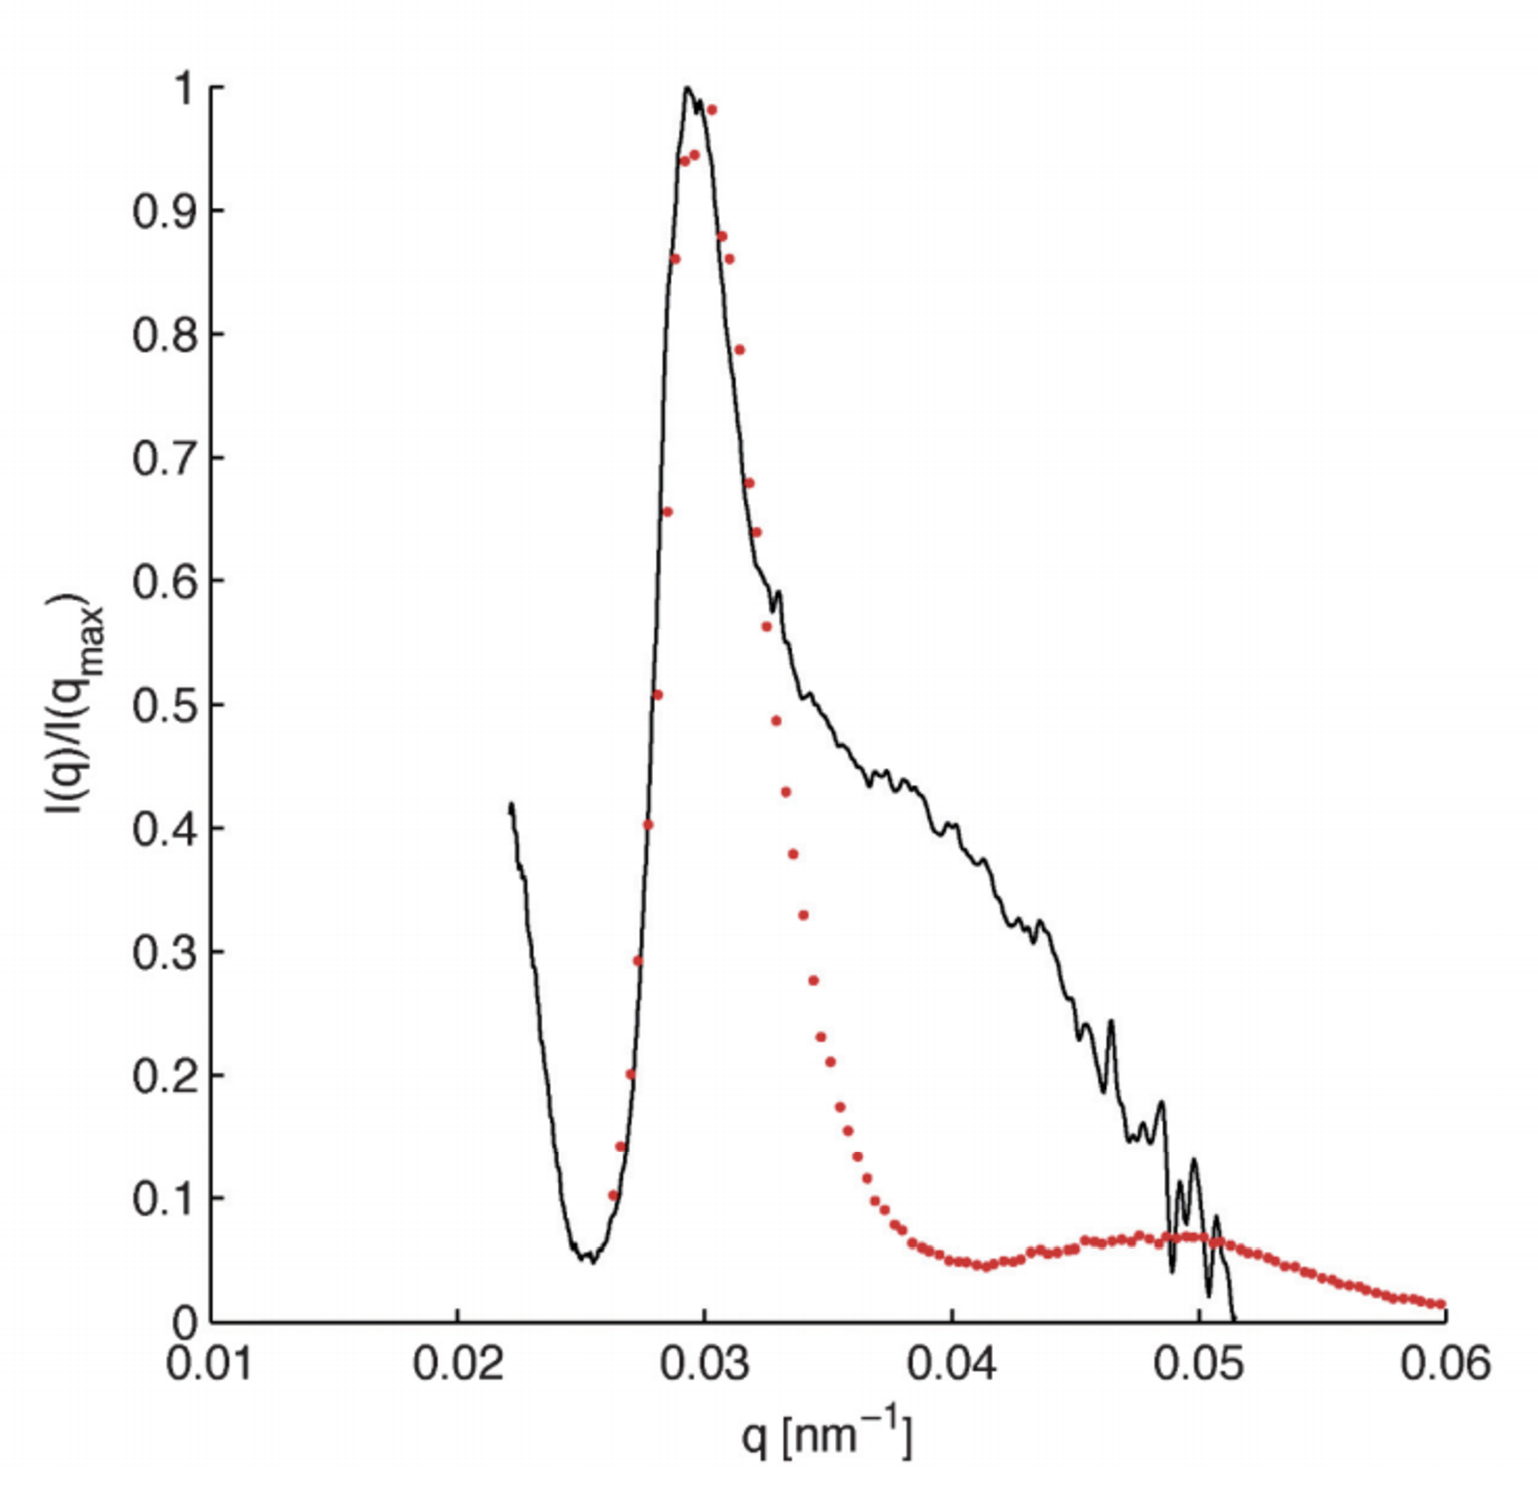
\includegraphics[width=4in]{figures/cmaynanacombined.pdf}
\caption{\label{fig:cotingacombined} \emph{Azimuthal average of SAXS pattern combined with optical reflection spectrum.}
	From Ref.~\cite{Dufresne:2009p6342}.}
\end{figure*}

Combining structural information from SAXS with optical scattering measurements reveals that single scattering is primarily responsible for the color.
In Figure~\ref{fig:cotingacombined}, we directly compare an optical reflection spectrum (black line) to the azimuthal average of the SAXS pattern in Figure~\ref{fig:cotingaSAXS} (red dots) by plotting the reflected intensity as a function of wavevector 
\begin{equation}\label{eqn:optical-to-q}
q = \frac{4\pi n_{e}}{\lambda}\cos{(\theta_m/2)},
\end{equation}
where $n_{e}$ is the effective refractive index of the material;  $\theta_m$ is the angle between illumination and detection, taking into account refraction at the film surface; and $\lambda$ is the wavelength of light in vacuum.
In general, the scattering intensity depends on wave vector, $q$, with the quantity $I(q)$ fully describing the spatial dependence of singly scattered light.
Therefore, Eqn.~\ref{eqn:optical-to-q} is a more general form of Bragg's Law (Eqn.~\ref{eqn:Bragg}), which only indicates the values of $q$ where scattering is strongest.
The index contrast between air and the protein matrix of the feathers for X-rays is very small, consequently, the scattering pattern we image in SAXS is the result of singly scattered photons.
The fact that the first peaks from both measurements have nearly the same shape indicates that singly scattered photons in the optical range are responsible for the color \cite{Dufresne:2009p6342}.
The disagreement of the two curves at higher $q$ can be attributed to multiple scattering events \cite{Noh:2010}.
The first peaks of both measurements have nearly the same position when a value of 1.25 is used for $n_e$, indicating that air occupies 62\% of the volume in this structure.

The goal of the next section is to design and assemble a material composed of spherical colloidal particles with the same structural and optical properties as these bird feathers.


\section{Self-Assembly of an Isotropic Structure of Spheres}

In recent years, periodic biological structures have provided inspiration for groups trying to make photonic materials \cite{Parker:2004p11036, Parker:2007p11434}. 
Much of this work has been motivated by producing a photonic band gap \cite{Yablonovitch:1987p1809, Joannopoulos:2008p11516, Noda:2003p11561, MSoukoulis:2001p11651, Kinoshita:2008p10935, Muller:2000p5865}. 
However, Nature's alternative design, based on isotropic structures is just starting to be explored \cite{Hallam:2009p11443, Takeoka:2009p10174, Saranathan:2011}. 
Hallam \emph{et al} have used biomimetic random structures to make ultra-thin mineral coatings that are brilliant white.
Takeoka \emph{et al} recently showed  that a wide range of colors with very little angle dependence can be produced by microgel dispersions.
In this section, we describe the self-assembly of biomimetic isotropic films which display structural color that is amenable to  potential applications in coatings, cosmetics, and textiles.
We find that isotropic structures with a characteristic length-scale comparable to the wavelength of visible light can produce structural color when wavelength-independent scattering is suppressed.

\begin{figure*}[htbp]
\centering
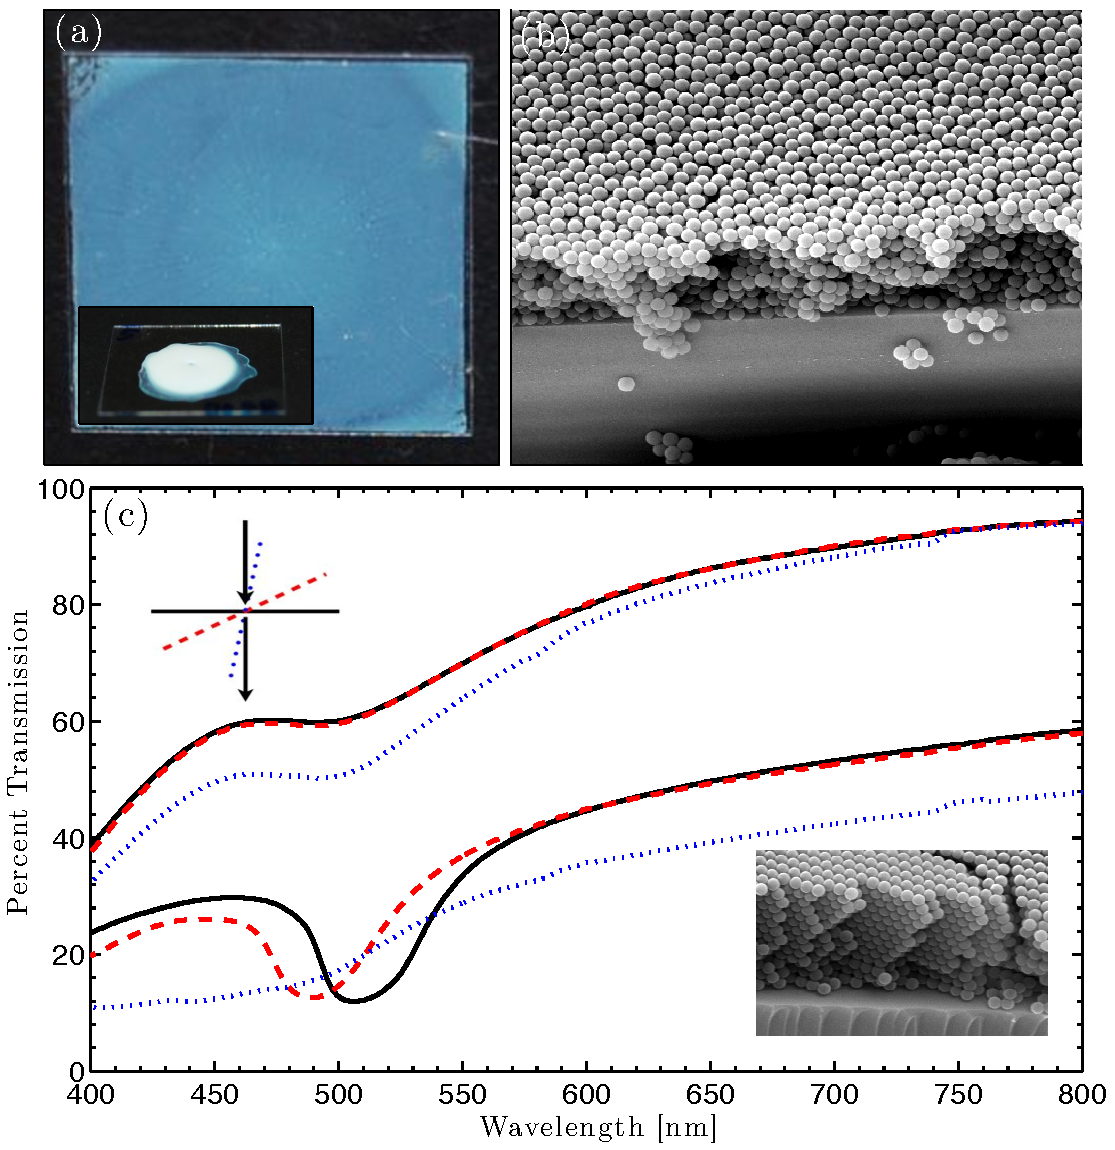
\includegraphics[width=.9\textwidth]{figures/transmission_100128.pdf}
\caption{\label{fig:transmission}\emph{Effect of disorder and order on optical properties.} 
	\emph{a)} Photograph of a film of 226 and 271 nm PS spheres spin-cast onto an 18 $\times$ 18 mm glass coverslip. \emph{Inset}: Photograph of a dried sessile droplet. 		\emph{b)} Side-view SEM image a similar film. The field of view is 8.8 $\mu$m wide. 	\emph{c)} The top set of curves show the transmission spectra for the isotropic film pictured in (a).The bottom set of curves show the results of the same measurement performed with a crystalline sample, made by spin-casting 226 nm PS spheres. The data were taken with the sample normal to the optical path (solid line), at an angle of 30$^{\circ}$ (dashed red line), and at an angle of 80$^{\circ}$ (dotted blue line), represented schematically in the upper left hand corner. \emph{Inset}:  Side-view SEM image of a crystalline sample, the field of view is 5.3 $\mu$m wide.}
\end{figure*}

We make two types of films that are structurally-colored by exploiting the self-assembly of colloidal polymer nanoparticles.
The first type of sample is a thin film on a glass coverslip produced by spin casting an aqueous suspension of spheres (Figure~\ref{fig:transmission}a).
While monodisperse dispersions form anisotropic polycrystalline films, as shown in the inset of Figure~\ref{fig:transmission}c, a mixture of two sizes of spheres ensures an isotropic structure as shown in Figure~\ref{fig:transmission}b.
The blue-green film  in Figure~\ref{fig:transmission} is made from a bidisperse suspension of polystyrene (PS) spheres with mean diameters of 226 and 271 nm and polydispersity 2\% in equal volume fractions.

The synthesis of monodisperse PS spheres using surfactant-free emulsion polymerization is described in Appendix~\ref{chap:synthesis:ps} and in Ref.~\cite{CHONDE:1981p1047}.   
After synthesis, particle suspensions are washed by centrifugation and resuspension at least three times with DI water.  
After washing, the suspensions are adjusted to $\phi_{PS}$ = 0.3.  
The sizes of particle are determined by scanning electron microscopy (SEM) image analysis using a Philips XL-30 ESEM with an accelerating voltage of 10 kV, after being coated with a thin layer of gold.

To prepare bidisperse suspensions, equal volumes of two monodisperse suspensions are mixed by pipetting approximately 20 times and vortexing for at least 30 seconds.  
Prior to spin casting for thin films or water evaporation for thick films, the suspensions are sonicated for at least 20 minutes to break up any aggregates.  
Thin films are spin cast onto glass coverslips cleaned with ethanol using a Headway Research, Inc. PWM32-PS-R790 spin coater.  
Typical spin speeds are between 500 and 5000 RPM, the spin speed and viscosity of the suspension determine the final thickness of the film \cite{Jiang:2004p8684}. 

The side-view SEM in Figure~\ref{fig:transmission}b is of a film comparable to the one in Figure~\ref{fig:transmission}a and shows that there is no long range order, it also reveals a representative thickness of 2.3$\pm$0.2 $\mu$m.  

The optical properties of isotropic and crystalline films are quite different, even for samples prepared with very similar particles.
We compare the transmission spectra of isotropic and crystalline samples in Figure~\ref{fig:transmission}c.
Transmission spectra are measured using a Hitachi U-2001 spectrophotometer.
The isotropic film is the same one pictured in Figure~\ref{fig:transmission}a, the crystalline film is composed solely of the 226 nm spheres.
Both samples show a dip near 500 nm at normal incidence.
However, when the angle of incidence is changed, the spectral position of the dip for the crystalline sample shifts and eventually disappears.  
In contrast,  the position of the dip for the isotropic sample does not move.
This illustrates the trade-off in optical performance between crystalline and isotropic structures: while the crystalline film has more pronounced features at some angles, the isotropic film performs consistently over a wide range of angles.


To quantify the structure of the films, we perform small-angle X-ray scattering (SAXS) measurements on samples composed of spheres with mean diameters of 226 and 265 nm with 2\% polydispersity, spin-cast on kapton tape.
A typical scattering pattern is shown in Figure~\ref{fig:structure}a.
The pattern is dominated by a ring of uniform intensity, indicating that there is a well-defined length scale with no preferred direction --- the structure is isotropic with short-range order.
The azimuthal average of this pattern is shown in Figure~\ref{fig:structure}b, along with the expected scattering intensity from simulations of jammed packings of bidisperse spheres with size and number ratios that match our experimental system.
The position of the first peak in $I(q)$ occurs at $q_0=$ 0.03 nm$^{-1}$ for both simulation and experiment.
The full width at half maximum (FWHM) of the first peak, $\Delta q$, characterizes the range of spatial order $\xi = 2\pi/\Delta q$ = 870 nm.
In powder crystallography, $\xi$ describes the crystal domain size, here, $\xi$ is only a few particle diameters.

SAXS measurements of biomimetic samples are carried out at beamline X9 at the NSLS, Brookhaven Naitonal Laboratory, using a Rayonix Mar 165 CCD detector. 
The X-ray energy is 7 keV (a wavelength of 1.771 \AA) and the sample-to-detector distance is ~5 m. 
The conversion from the detector image to reciprocal space is calibrated using the diffraction pattern from a standard silver behenate sample ($q_0=$ 0.1076 \AA$^{-1}$). 
The first ring from silver behenate is out of the angular range covered by the detector at 7 keV, therefore the standard pattern was collected with the same scattering geometry but at an X-ray energy of 15.65 keV (0.792 \AA). 
The finite beam size at the detector corresponds to FWHM $q$ resolution of 0.00045 \AA$^{-1}$, which is $\sim$17$\%$ of the width of the fringe produced by the spheres ($\pi/120$ nm $\approx$ 0.0026 \AA$^{-1}$).
Biomimetic samples for SAXS measurements are prepared on 0.0025"-thick Kapton Tape, purchased from McMaster-Carr (catalog no. 7648A33).

To simulate the structure of our samples, we create mechanically stable packings of bidisperse frictionless spheres in cubic cells with periodic boundary conditions using a simulation protocol in which we successively compress/decompress soft particles and then apply conjugate gradient energy minimization until particles are just at contact (up to a prescribed energy threshold) \cite{Gao:2006p061304}.  
The energy threshold, initial packing fraction $\phi_0$, and increment in $\phi$ are set to $10^{-8}$, $0.2$ and $10^{-4}$, respectively.  
We select particle size and number ratios to match the experiments. 
From $50$ independent initial configurations, we obtain an average packing fraction $\phi_J = 0.63$, which is relatively insensitive to the specific parameters of the packing-generation protocol.  
From the particle centers, we calculate the partial, $S_{ll}(q)$, $S_{ss}(q)$, and $S_{ls}(q)$, and total structure factor 
\begin{equation}\label{eqn:structure-factor}
S(q) = x_l S_{ll}(q) + x_s S_{ss}(q) + 2\sqrt{x_l x_s} S_{ls}(q),
\end{equation}
 where $l,s$ signify large or small particles, $x$ is the number fraction of the indicated particle, and $q$ is the wavevector. 
The partial structure factors and the theoretical form factors for each sphere size are used to calculate the total scattering intensity 
\begin{equation}\label{eqn:total-scattering}
I(q) \propto x_l S_{ll}(q) F_l^2(q) + 2\sqrt{x_l x_s}S_{ls}(q) F_l(q) F_s(q) + x_s S_{ss}(q) F_s^2(q).
\end{equation}

	
\begin{figure*}[htbp]
\centering
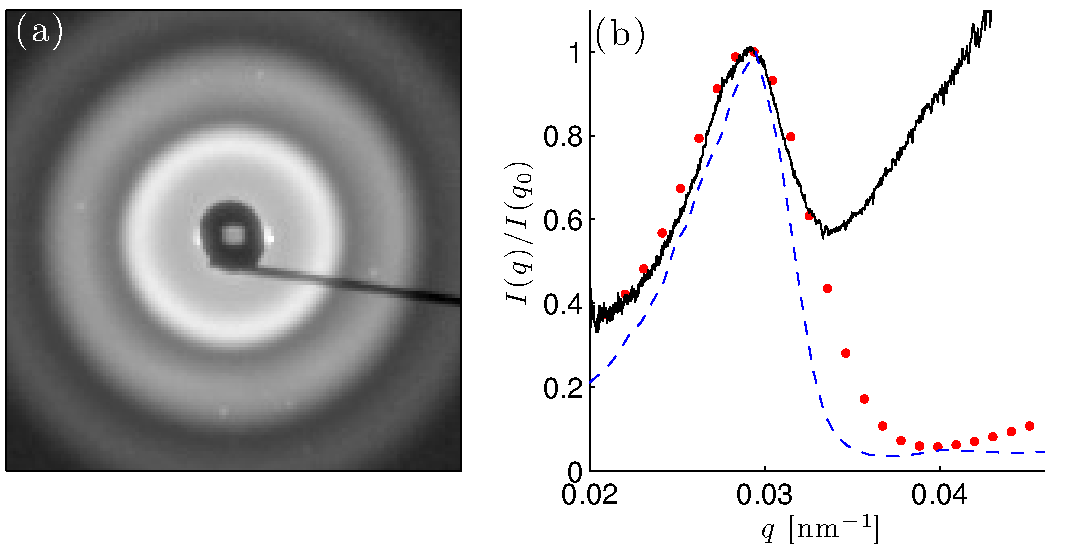
\includegraphics[width=.9\textwidth]{figures/structure_100128.pdf}
\caption{\label{fig:structure} \emph{Structure of isotropic films.}
	\emph{a)} SAXS pattern from an isotropic film, the field of view is 0.15 nm$^{-1}$ and the gray values are logarithmic in intensity.
	\emph{b)} The azimuthal average of the experimental (red dots) and numerical (blue dashed line) scattering pattern.  The black line is optical reflectivity data taken at an angle of 10$^{\circ}$ (experiment geometry shown in Figure~\ref{fig:qseries}) converted to q-space using an effective refractive index of $n_{e}=1.24$.}
\end{figure*}

We directly compare optical reflectivity measurements to SAXS measurements in Figure~\ref{fig:structure}b by plotting the reflected intensity as a function of wavevector using Eqn.~\ref{eqn:Bragg}.
The peaks from both measurements match when $n_{e} =$ 1.24.  We apply the Maxwell-Garnett equation,
\begin{equation}\label{eqn:maxwell-garnett}
n_{e} = n_{air}\left(\frac{2n_{air}^2 + n_{PS}^2 + 2\phi(n_{PS}^2 - n_{air}^2)}{2n_{air}^2 + n_{PS}^2 - \phi(n_{PS}^2 - n_{air}^2)}\right)^{1/2}
\end{equation} 
to calculate the volume fraction of spheres, $\phi =$ 0.46$\pm$0.04, where $n_{PS}$ is the index of refraction of the spheres, taken to be 1.58, and $n_{air}$ is taken to be 1.00.  
The optical reflection and scattering spectra were performed with a custom-built setup in Hui Cao's laboratory described in detail in Noh \emph{et al} \cite{Noh:2009AM}.


\section{Suppression of Multiple Scattering by Absorption}

Isotropic films can produce structural color with little angle dependence, but the film thickness  critically affects its color, as seen in the inset of Figure~\ref{fig:transmission}a.
Here, we cast a thick film by  drying  a sessile droplet of the same suspension used to make the thin films.
In thick regions near the center, the film appears white.
In thin sections near the edge, it appears blue-green.
This thickness dependence can be understood in the following way.
The film preferentially scatters wavelengths corresponding to the peak in $I(q)$.
In a thin film, only these wavelengths will be scattered to the detector resulting in a structural color.
In a thick film, all wavelengths are scattered multiple times and reach the detector.

The sensitivity of the color to the film thickness requires well-controlled casting procedures which increase the cost and limit the coated area.
Therefore, for many potential applications it is necessary to eliminate the thickness-dependence.
We address this by introducing broadband absorption to the bulk of the films.
The absorption length plays a similar role as the thickness: it limits the path length of light through the film by absorbing photons that do not get scattered within a small distance from the surface. 
Thus, only wavelengths with the strongest scattering will escape the film before being absorbed.

\begin{figure*}[htbp]
\centering
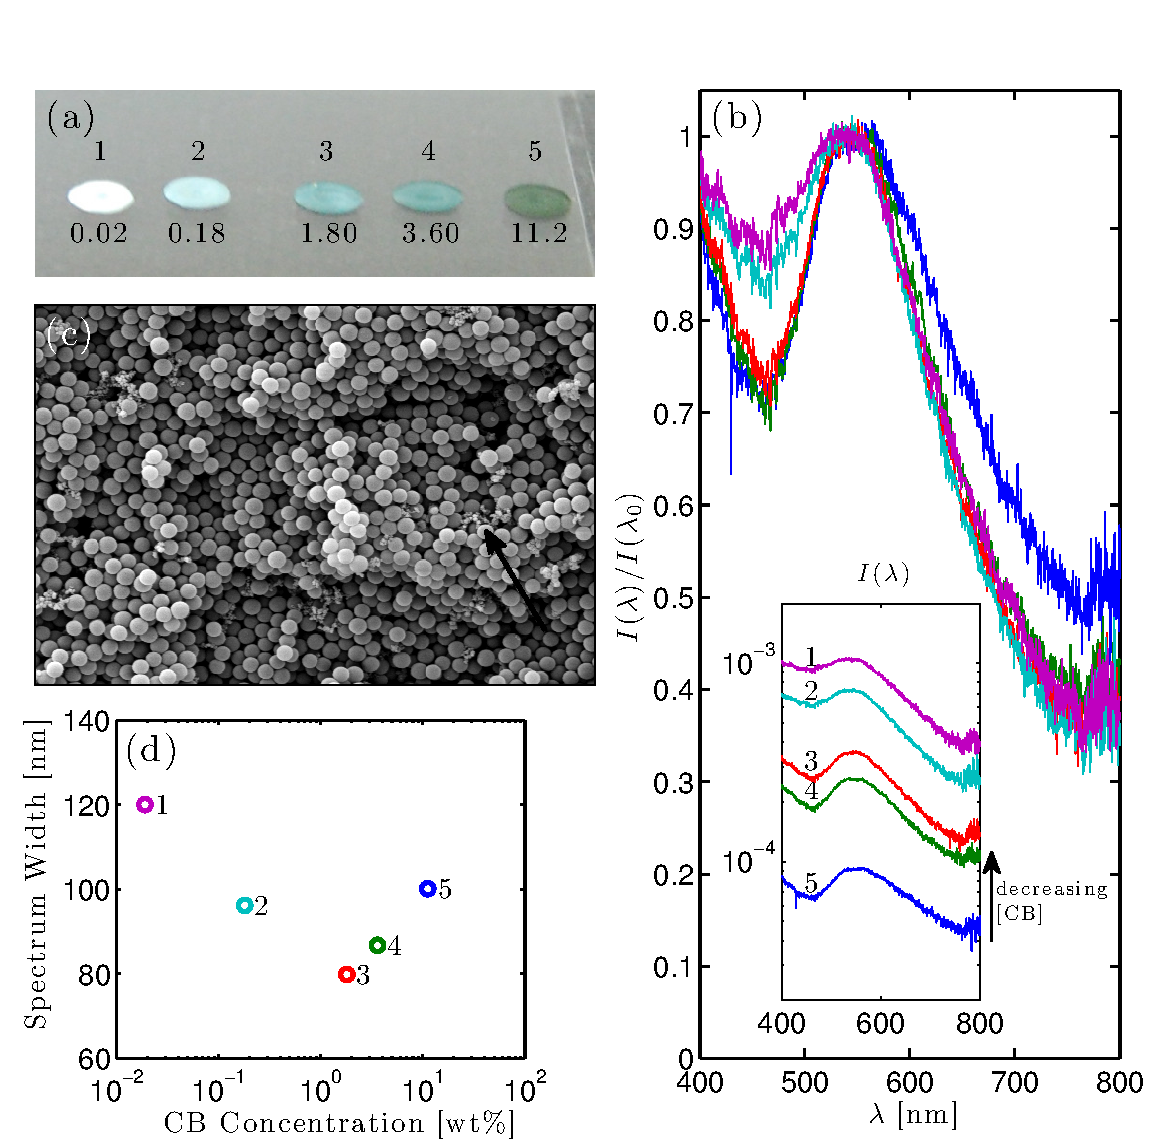
\includegraphics[width=.9\textwidth]{figures/carbonblack_100128.pdf}
\caption{\label{fig:carbonblack} \emph{Optimizing color by adding absorption.} 			\emph{a)} Photograph of five drop-cast films of 226 and 265 nm PS spheres containing carbon black.  Sample numbers and [CB] in wt$\%$ appear above and below the samples, respectively. 
	\emph{b)} Normalized optical scattering spectra recorded at an angle of 20$^{\circ}$ (experiment geometry shown in Figure~\ref{fig:qseries}) for the five samples in (a). \emph{Inset}: Non-normalized scattering spectra for the same samples. 
	\emph{c)} SEM image of the interior region of sample 3, the field of view is 7.8 $\mu$m wide, a piece of CB is indicated with an arrow. 
	\emph{d)} The width of the spectra for each sample in (a) at $I(\lambda)/I(\lambda_0) = 0.90$}  
\end{figure*}

We make a series of thick films with different absorption lengths by drop-casting films with varying concentrations of carbon black.
The photo in Figure~\ref{fig:carbonblack}a illustrates the effect of adding carbon black on the color of the material.
From left to right, the concentration of carbon black, [CB], is increased.
Intuitively, one might expect a mixture of black and white to make gray, but here they make blue-green over a range of [CB].
The plot in Figure~\ref{fig:carbonblack}b shows the normalized optical scattering spectra for these five samples.
As [CB] is increased from 0.02 wt\% to 1.80 wt\%, the contrast between scattered intensity at the peak and shorter wavelengths is increased, improving the color of the sample.
When [CB] = 11.2 wt\%, the scattered intensity is reduced by a factor of ten compared to the brightest sample (inset in Figure~\ref{fig:carbonblack}b), and the film appears dark gray.
The reflectance peak is narrowest for [CB] = 1.80 wt\% (Figure~\ref{fig:carbonblack}d), and indeed this sample has a distinct blue-green color.
Table~\ref{table:carbonblack} lists the [CB] for each sample and the corresponding extinction length: the extinction length is extrapolated from measurements of aqueous suspensions of CB.
Interestingly, the extinction length for sample 3 is 1.3 $\mu$m, which is comparable to the thickness of the thin film pictured in Figure~\ref{fig:transmission}a.

The carbon black suspension are prepared by mixing Cabot Vulcan XC72R GP-3919 carbon black in DI water at [CB] = 4.2 wt$\%$ with 1 wt$\%$ Pluronic F108 to stabilize the CB.  
Different volumes of the CB suspension are added to the bidisperse suspensions of spheres to produce samples with different final [CB].
To estimate the extinction lengths quoted in Table~\ref{table:carbonblack} and in Figure~\ref{fig:carbonblack}, the transmission spectra of aqueous suspensions of CB are measured using an Ocean Optics USB 650 Red Tide spectrometer.
Suspensions ranging from 8$\times$10$^{-5}$ to 2$\times$10$^{-2}$ wt$\%$ are used.  
Measurements are made with three different path lengths: 1 cm, 0.04 cm, and 0.03 cm.
The extinction length for all path lengths is proportional to [CB]$^{-1}$, as shown in Figure~\ref{fig:carbon-black-extinction}, allowing us to extrapolate the extinction length to the [CB] range used in our thick film samples.
We use extinction instead of absorption because this measurement does not discriminate between absorbed and scattered light.

\begin{figure*}[htbp]
\centering
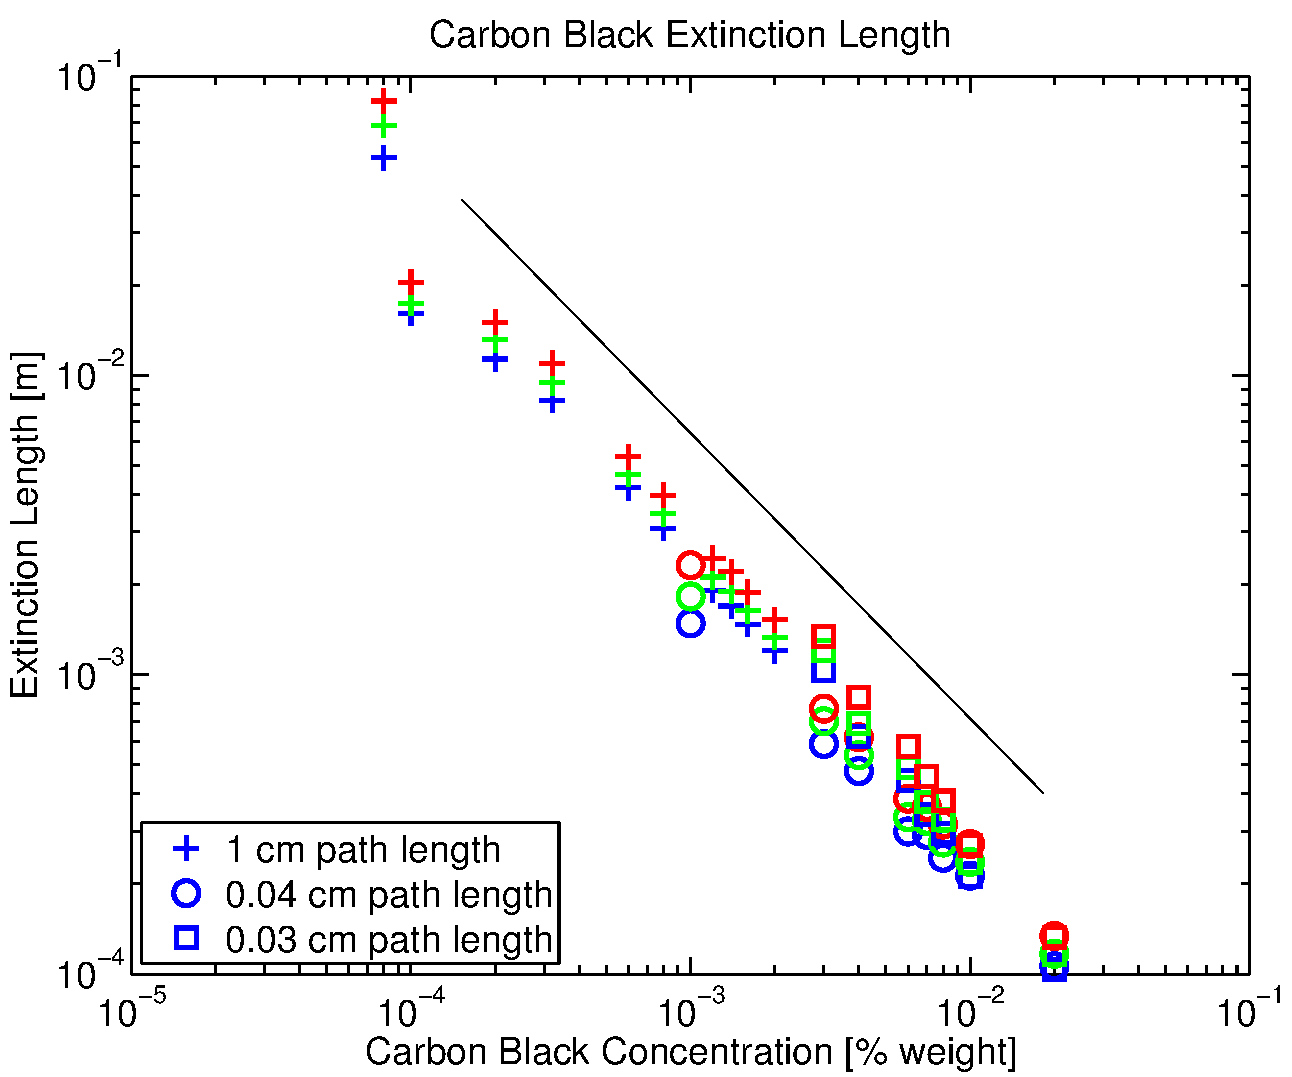
\includegraphics[width=.9\textwidth]{figures/carbonblackextinctionlength.pdf}
\caption{\label{fig:carbon-black-extinction}\emph{Carbon black extinction length is inversely proportional to the concentration of [CB].}
}
\end{figure*}

\begin{table}[htbp]\footnotesize
\centering
\caption{Carbon Black Extinction Length}
\begin{center}
\begin{tabular}{c c c}
Sample & [CB] [wt\%] & Extinction Length [m] \\
\hline
1 & 0.02 & 1.3$\times$10$^{-4}$\\
2 & 0.18 & 1.3$\times$10$^{-5}$\\
3 & 1.80 & 1.3$\times$10$^{-6}$\\
4 & 3.60 & 6.5$\times$10$^{-7}$\\
5 & 11.2 & 2.1$\times$10$^{-7}$\\
\end{tabular}
\end{center}
\label{table:carbonblack}
\end{table}


The thick films with CB are not iridescent under omnidirectional illumination, but, under directional illumination, the peak wavelength scattered does change slightly when the angle between illumination and detection is varied \cite{Noh:2009AM}. 
Since the colors are the result of single scattering, the position of the scattering intensity maximum does not vary with respect to $q$, as demonstrated by the spectra in Figure~\ref{fig:qseries}.
The red dots connected by a red line in Figure~\ref{fig:qseries} represent the azimuthal average of the SAXS pattern for a sample with the same [CB] prepared on kapton tape.  The peaks from the optical and SAXS measurements match when $n_{e} = $ 1.29, implying that $\phi_{s}$ = 0.54$\pm$0.05.
The higher value of $\phi_{s}$ for the thick films relative to the thin films of the previous section is most likely the result of the different quench-rates used to make the samples.
In the spin casting of thin films, the water evaporates within seconds, while water evaporates from the thick films over a few hours, allowing particle rearrangement which leads to a higher $\phi_s$.
In the thick film, we find that $\xi = $ 940 nm, only a few particle diameters.


\begin{figure*}[htbp]
\centering
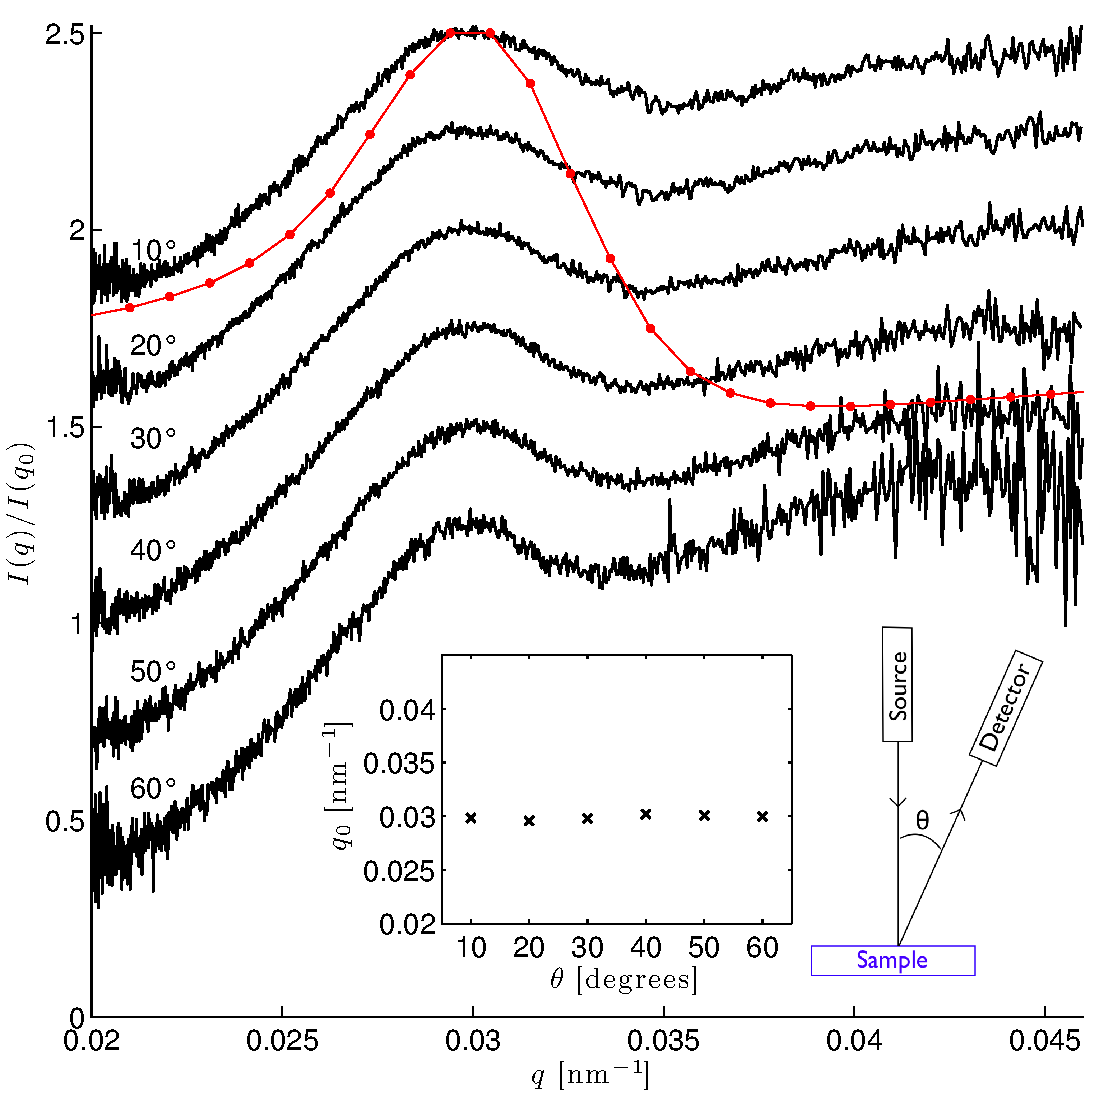
\includegraphics[width=.9\textwidth]{figures/qseries_100128.pdf}
\caption{\label{fig:qseries} \emph{Color is the result of single scattering.} 			Normalized reflectance spectra taken over a range of angles and converted to q-space for sample 2 in Figure~\ref{fig:carbonblack} (black lines), and the azimuthal average of the SAXS pattern for a similar sample (red dots). The spectra have been vertically offset for clarity. \emph{Inset}: Position of the peak as a function of angle. \emph{Schematic}: the source and sample are fixed and the detector is rotated.}
\end{figure*}


These isotropic films mimic the essential optical properties of bird feathers that have structural color from isotropic nanostructures.
A photograph of an example of these feathers from the crown of \emph{Lepidothrix coronata} is shown in Figure~\ref{fig:birdcomparison}a, and a transmission electron micrograph (TEM) of the color-producing structure is shown in Figure~\ref{fig:birdcomparison}b.
Normalized $I(q)$ from both \emph{L. coronata} and sample 2 from Figure~\ref{fig:carbonblack} are plotted as a function of $q/q_{0}$ in Figure~\ref{fig:birdcomparison}c.
SAXS measurements of the feathers are carried out at beamline 8-ID-I at the APS, Argonne National Labs, as described in Dufresne \emph{et al} \cite{Dufresne:2009p6342}.
The SAXS patterns reveal similar structures out to the third peak in $I(q)$.
Beyond that, the thick film has additional peaks that arise from the uniformity of the spheres used in the sample.
We compare the performance of the feathers and films by plotting optical scattering spectra for both at 20$^\circ$ in Figure~\ref{fig:birdcomparison}d.
The scattered optical intensity peak for \emph{L. coronata} is narrower than the film: the full-width at $I(\lambda)/I(\lambda_0) = 0.90$ is 49 nm for the feather and 82 nm for the film. 
Similarly, \emph{L. coronata} has a narrower first peak in $I(q)$.
\emph{L. coronata} also displays less scattering at shorter wavelengths.
This may be due to a significant difference in the two structures: the feathers have spheres of air in a high-index of refraction background whereas the films have spheres of a high-index in a background of air.


\begin{figure*}[htbp]
\centering
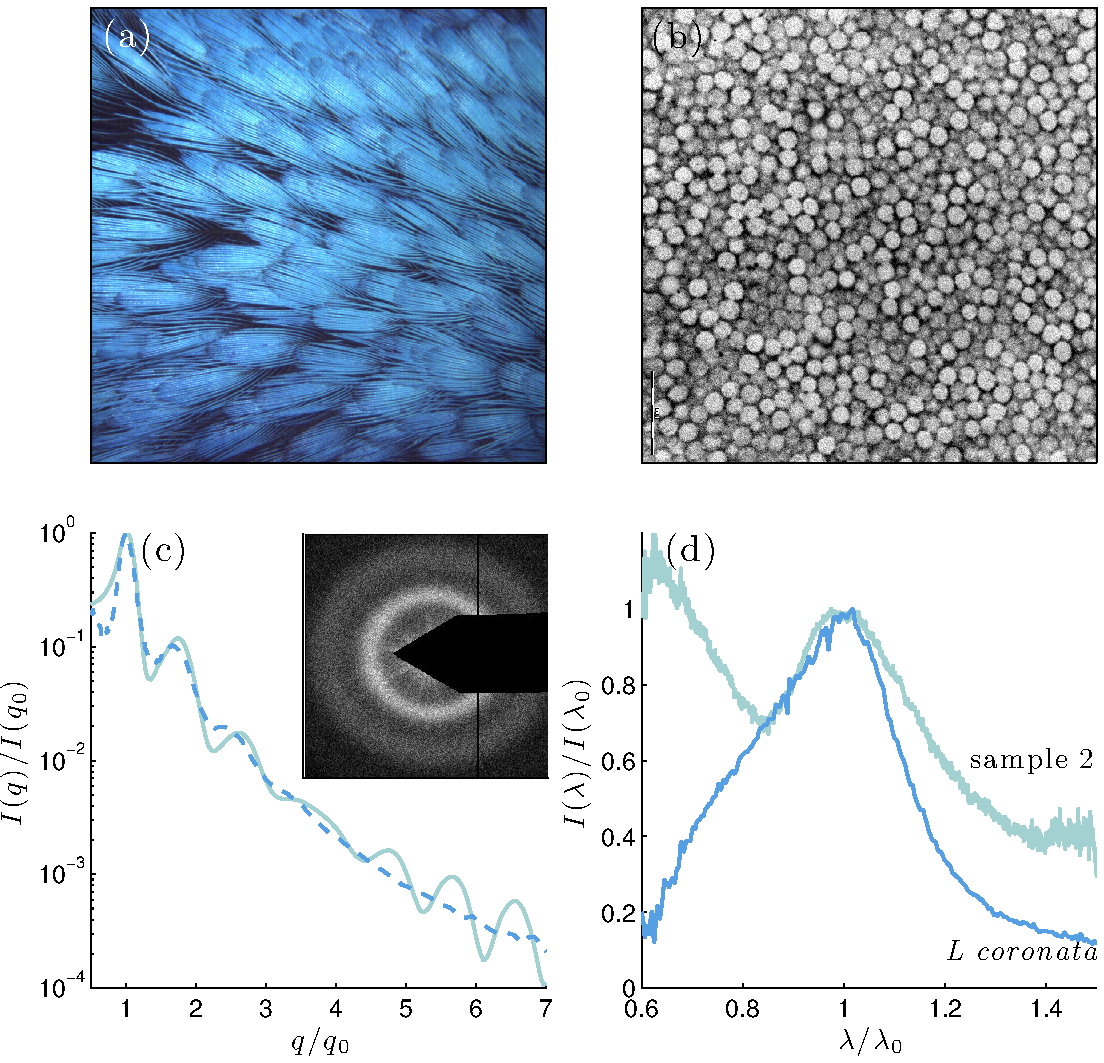
\includegraphics[width=.9\textwidth]{figures/birdcomparison_100128.pdf}
\caption{\label{fig:birdcomparison} \emph{Comparison with feathers.} 	
	\emph{a)} Photograph of crown feathers from \emph{L. coronata}, the field of view is 1 cm. 
	\emph{b)} TEM image of air spheres in beta-keratin from \emph{L. coronata}, the field of view is 5.5 $\mu$m. 
	\emph{c)} Azimuthal averages from SAXS measurements of \emph{L. coronata} (dashed line) and a thick film with the same [CB] as sample 2 in Figure~\ref{fig:carbonblack} (solid line). \emph{Inset:} SAXS pattern from \emph{L. coronata}, the field of view is 0.14 nm$^{-1}$ and the gray values are logarithmic in intensity. 
	\emph{d)} Comparison of optical scattering data taken at an angle of 20$^{\circ}$ (experiment geometry shown in Figure~\ref{fig:qseries}) from \emph{L. coronata} and sample 2 from Figure~\ref{fig:carbonblack}.  The line colors correspond to the apparent color of the feathers and the thick film.}
\end{figure*}
